%!TEX program = xelatex
\documentclass[tikz, class=report]{standalone}
\usepackage[lining]{ebgaramond}%[StylisticSet={7,9}]
\usepackage[math-style=ISO, bold-style=ISO]{unicode-math}
\setmathfont{Garamond-Math.otf}
\usepackage{pgfplots}
\usepackage{import}
\makeatletter
  \def\input@path{%
    {../tex/}
    {../../tex/}
    {../../../tex/}
    {../../../../tex/}
  }
\makeatother

\usetikzlibrary{positioning}
\usetikzlibrary{arrows.meta}

\newcommand{\bardist}{3.5}

\newcommand{\xleg}{-2}
\newcommand{\yleg}{-2}
\newcommand{\boxh}{0.2}
\newcommand{\boxl}{0.7}
\newcommand{\legsepy}{0.4}
\newcommand{\legsepx}{3.5}

\newcommand{\units}{$5 \cdot 10^{-3} \frac{\mbox{cts}}{\mbox{keV}\cdot\mbox{kg}\cdot\mbox{yr}}$}
\newcommand{\unitsbis}{$2 \cdot 10^{-3} \frac{\mbox{cts}}{\mbox{keV}\cdot\mbox{kg}\cdot\mbox{yr}}$}

\definecolor{vib-blue}   {RGB}{  0, 119, 187}
\definecolor{vib-cyan}   {RGB}{ 51, 187, 238}
\definecolor{vib-teal}   {RGB}{  0, 153, 136}
\definecolor{vib-orange} {RGB}{238, 119,  51}
\definecolor{vib-red}    {RGB}{204,  51,  17}
\definecolor{vib-magenta}{RGB}{238,  51, 119}
\definecolor{mut-olive}  {RGB}{153, 153,  51}
\definecolor{mut-sand}   {RGB}{221, 204, 119}
\definecolor{mut-indigo} {RGB}{51,   34, 136}

\begin{document}
  \begin{tikzpicture}
    \tikzset{
      legbox/.style={opacity=0.8, draw=black, minimum height=\boxh cm, minimum width=\boxl cm, above right},
      labelbox/.style={font=\small},
      location/.style={right, rotate=90, font=\small},
      myhead/.style={{Bar[width=3pt]}-{Bar[width=3pt]}, thick},
      pics/location/.style args={#1,#2,#3}{code={%
        \draw (#1,#2) -- ++(0,0.4) node[above right=-0.7mm and 1.8mm, rotate=90, font=\small] {#3};%
      }}%
    }

    % bars
    \node at (5,0.5+2*\bardist) {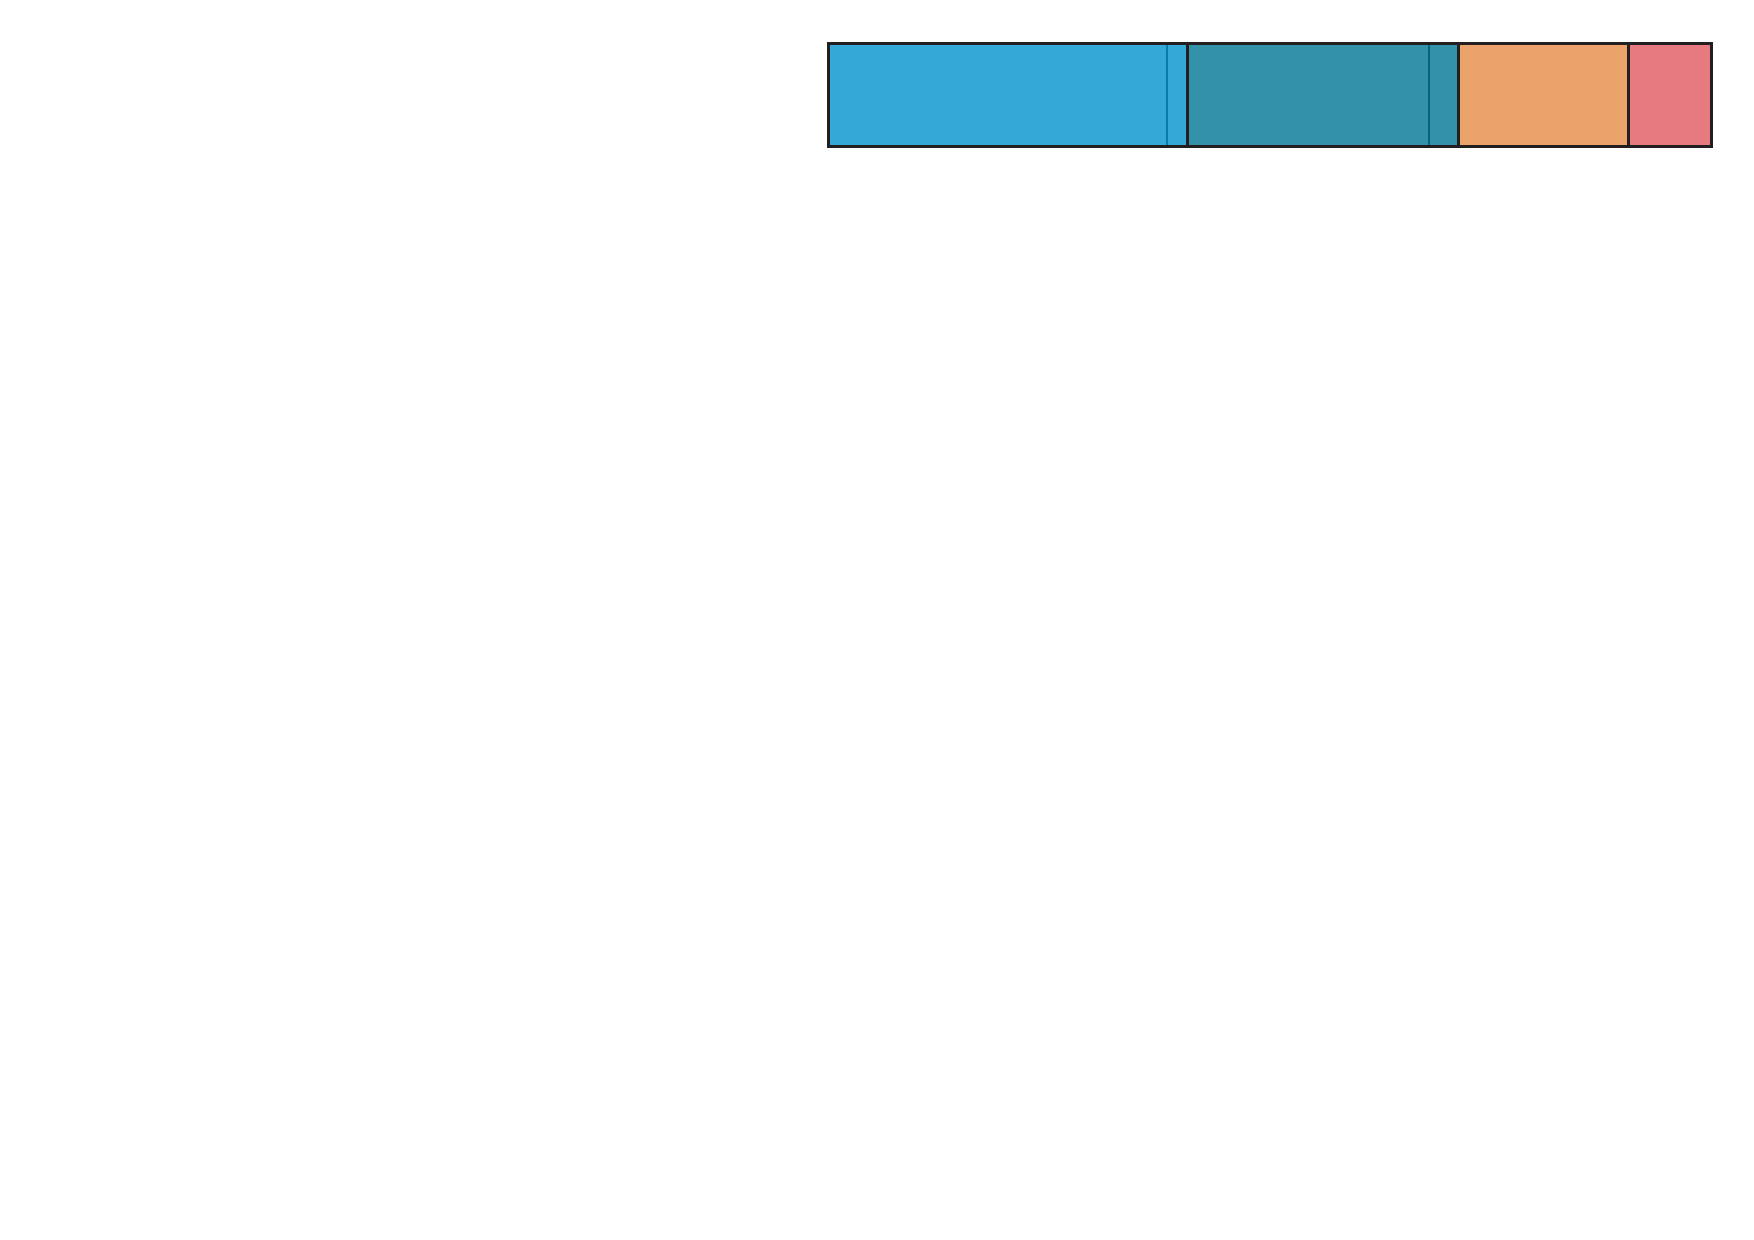
\includegraphics[width=10cm, height=1cm]{BI-boxes-E1plusE2.pdf}};
    \node at (5,0.5+\bardist)   {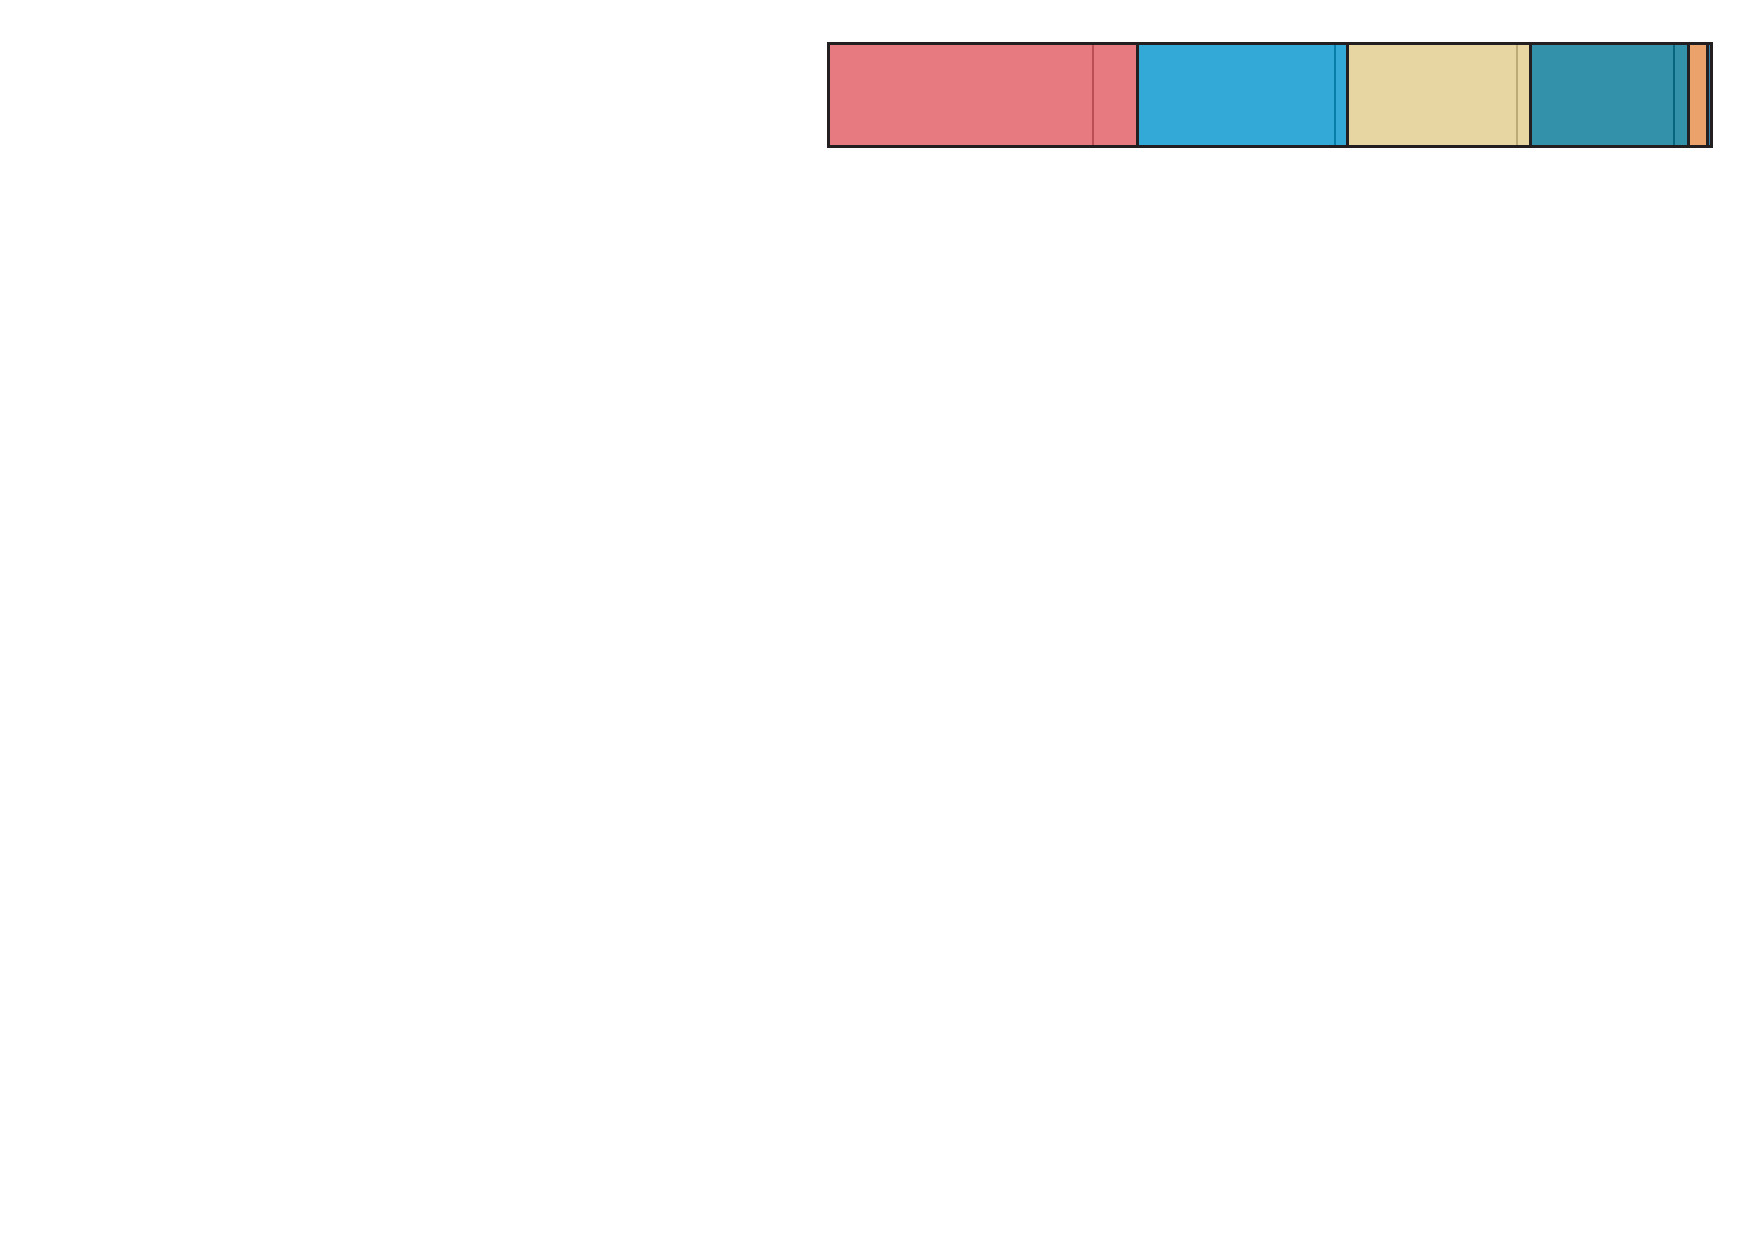
\includegraphics[width=10cm, height=1cm]{BI-boxes-enrBEGe.pdf}};
    \node at (5,0.5)            {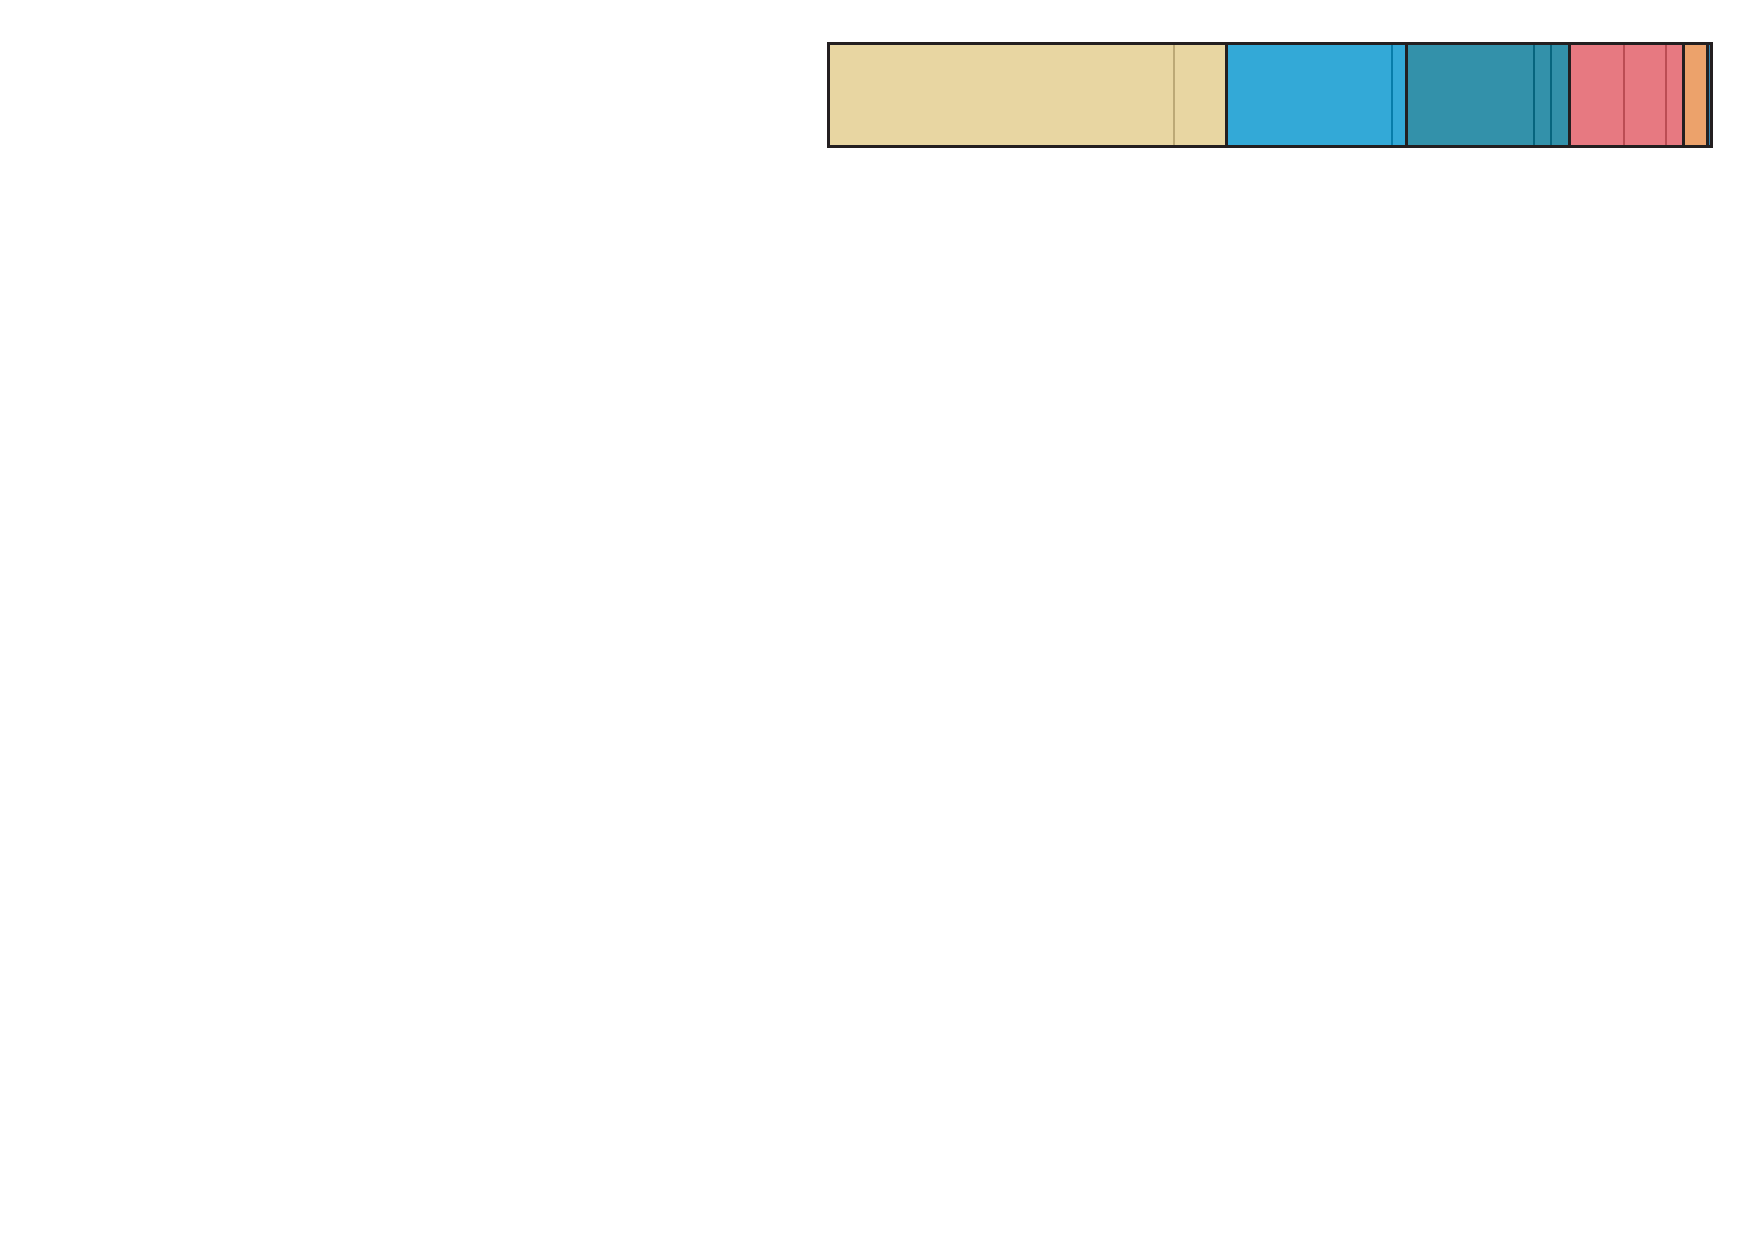
\includegraphics[width=10cm, height=1cm]{BI-boxes-enrCoax.pdf}};

    % names
    \node at (-1,0.5+2*\bardist) {\texttt{M2-enrGe}};
    \node at (-1,0.5+\bardist)   {\texttt{M1-enrBEGe}};
    \node at (-1,0.5)            {\texttt{M1-enrCoax}};

    % locations
    \draw pic {location={1.7,1+2*\bardist,cables}};
    \draw pic {location={3.5,1+2*\bardist,fibers}};
    \draw pic {location={3.85,1+2*\bardist,mini-shrouds}};
    \draw pic {location={5.5,1+2*\bardist,cables}};
    \draw pic {location={8,1+2*\bardist,cables}};
    \draw pic {location={9.3,1+2*\bardist,hom.}};
    \draw pic {location={9.75,1+2*\bardist,above arr.}};
    \draw (9.9,1+2*\bardist) -- ++(0,0.2) -- ++(0.2,0.4) -- ++(0,0.3) node[above right=-0.7mm and 2.5mm, rotate=90, font=\small] {n$^+$ (\textsc{SemiCoax})};%

    \draw pic {location={1.8,1+\bardist,n$^+$}};
    \draw pic {location={3.3,1+\bardist,out. ms}};
    \draw pic {location={4.7,1+\bardist,cables}};
    \draw pic {location={5.8,1+\bardist,mini-shrouds}};
    \draw (6.9,1+\bardist) -- ++(0,0.4) node[above right=-0.7mm and 2.3mm, rotate=90, font=\small] {degr.~$\alpha$};%
    \draw pic {location={7.85,1+\bardist,$^{210}$Po}};
    \draw pic {location={8.85,1+\bardist,cables}};
    \draw pic {location={9.65,1+\bardist,mini-sh.}};
    \draw (9.85,1+\bardist) -- ++(0,0.2) -- ++(0.2,0.4) -- ++(0,0.3) node[above right=-0.7mm and 2.5mm, rotate=90, font=\small] {cables};%

    \draw (2.4,1) -- ++(0,0.4) node[above right=-0.7mm and 2.3mm, rotate=90, font=\small] {degr.~$\alpha$};%
    \draw pic {location={4.2,1,$^{210}$Po}};
    \draw pic {location={5.5,1,cables}};
    \draw pic {location={6.45,1,mini-shrouds}};
    \draw pic {location={7.4,1,cables}};
    \draw (8.1,1) -- ++(0,0.2) -- ++(-0.2,0.4) -- ++(0,0.2) node[above right=-0.7mm and 2.5mm, rotate=90, font=\small] {mini-s.};%
    \draw pic {location={8.3,1,p$^+$}};
    \draw pic {location={8.7,1,n$^+$}};
    \draw pic {location={9.25,1,outside ms}};
    \draw pic {location={9.55,1,above array}};
    \draw pic {location={9.8,1,cables}};

    % scales
    \draw[myhead] (10-2.1723466,-0.3+2*\bardist) -- node[below] {\scriptsize\unitsbis} (10,-0.3+2*\bardist);
    \draw[myhead] (10-3.4676601,-0.3+\bardist)   -- node[below] {\scriptsize\units}    (10,-0.3+\bardist);
    \draw[myhead] (10-2.8521511,-0.3)            -- node[below] {\scriptsize\units}    (10,-0.3);

    % legend
    \node[legbox, fill=vib-teal] (214) at (\xleg,\yleg+2*\legsepy) {};
    \node[labelbox, right=0.1cm of 214] {$^{214}\mbox{Bi} + {^{214}\mbox{Pb}}$};
    \node[legbox, fill=vib-cyan] (208) at (\xleg,\yleg+\legsepy) {};
    \node[labelbox,right=0.1cm of 208] {$^{212}\mbox{Bi} + {^{208}\mbox{Tl}}$};
    \node[legbox, fill=vib-magenta] (42) at (\xleg,\yleg) {};
    \node[labelbox, right=0.1cm of 42] {$^{42}$K};

    \node[legbox, fill=vib-blue] (else) at (\xleg+\legsepx,\yleg+2*\legsepy) {};
    \node[labelbox, right=0.1cm of else] {$2\upnu\upbeta\upbeta + {^{228}\mbox{Ac}}$};
    \node[legbox, fill=mut-sand] (alpha) at (\xleg+\legsepx,\yleg+\legsepy) {};
    \node[labelbox, right=0.1cm of alpha] {$\upalpha$-events};
    \node[legbox, fill=vib-orange] (60) at (\xleg+\legsepx,\yleg) {};
    \node[labelbox, right=0.1cm of 60] {$^{60}$Co};
  \end{tikzpicture}
\end{document}
